\documentclass{article}
\usepackage{sdss2020} % Uses Times Roman font (either newtx or times package)
\usepackage{graphicx}

\title{Using neural ordinary differential equations to infer ecological interactions from time series data}

\author{Sebastian Nuxoll \\ MATH-437 \\ Mathematical Biology \\ {\tt nuxo8861@vandals.uidaho.edu}}

\begin{document}
\maketitle
\begin{abstract}
Understanding ecological interactions is important for effective conservation. One way to find interactions is to construct a differential equation model that fits the data, and analyze each term. It can be difficult to construct traditional differential equations that fit times series data when the underlying ecological interactions are unknown. A neural network can be used to fit differential equations to time series data, allowing us to build a model while minimizing initial assumptions about the base system.
\end{abstract}

\section{Introduction}

Population dynamics have always been central to the the study of ecology and natural resources. Time series data is one the most ubiquitous forms of data gathered in the field, but they can be hard to gleen meaning from. Researchers often want to find relationships between populations in the data. This is hard for two reasons. Firstly, there are a plethora of factors that contribute to changes in population, many of which aren't captured in a given dataset. This means that even comparatively strong models fit to time-series data will begin to stray from the data over time, making it hard to see if the models are representative of the data.

Using a system of differential equations to model the system resolves this issue, since the model is no longer based on time, but this bring its own issues. The traditional way to construct a differential equation model is to select effects and realtionships to use as terms in the differential equations. This means that the effects found by analyzing the model are going to be affected by the way the model was constructed in the first place. These "parametric" models lead to a trial-and-error approach where every effect has to be explicitly tested to see if it improves the model. This leads to inherently rigid and biased results.

One way to avoid these issues is to implement a model based on Neural Ordinary Differential Equations (NODEs) \cite{earlierpaper}. The use of Artificial Neural Networks (ANNs) to represent differential equations allows for an unbiased structure that can be easily fit using backpropagation. 

In this paper, I will be exploring how NODEs handle different datasets, and the effects of different activation functions on the process. Traditionally, a sigmoid-like function is used as an activation function for most ANNs, but this is necessarily the optimal approach for our NODEs because of their small depth. I will be testing which activation function is most optimal for two types of dataset: one two-species system of hare and lynx in the Hudson Bay area and one three-species system of a rotifer, flagellate, and algae in a lab.

\section{Methods}

\subsection{Neural Ordinary Differential Equations}
A NODE is a differential equation that is defined primarily by an ANN. They can be used to find interactions in time series data, since they make minimal assumptions about the relationships between populations. I will use perceptrons as the ANNs of my NODES. A perceptron is a series of matrix multiplications and vector transformations that takes a set of inputs and provides a single output \cite{backproppaper}. 

Perceptrons are comprised of several layers. There is generally at least one hidden layer, which is comprised of a matrix of weights, a bias vector, and an activation functions. The input of the layer is multiplied by the weight matrix, then added with the bias vector, an finally, the activation function is applied to each value of the resulting vector. This vector is then passed to the next layer. The final layer is called the output layer, and is comprised of just a weight matrix and a bias vector. I will be using perceptrons with a single hidden layer, as described by the expression below \cite{backproppaper}.
$$f_p(y, W_1, W_2, b_1, b_2)=W_2(f_\sigma(W_1y+b_1))+b_2$$
Since we only have $2$ input values, one hidden layer should be enough to capture most of the dynamics of the system.

\subsection{Backpropagation}
The advantage of using an ANN is that there is a large amount to parameters that can be used to closely fit the model to data. Each parameter is modified based on each data point in the dataset in a process called backpropagation. For each given data point, a cost function can be constructed that takes all of our parameters, and outputs the difference of squares of the output based on the parameters and the actual output from the datapoint.
$$C_y(W_1, W_2, b_1, b_2)=f_p(y_{in}, W_1, W_2, b_1, b_2)^2-y_{out}^2$$
The parameters can be adjusted to better fit the data by subtracting the gradient of the cost function from the at each point \cite{backproppaper}. The gradient of a single-layer perceptron is described below, where $x$ is the data input, $m$ is the value of the middle layer, and $y^*$ is the output of the ANN:
$$\frac{\partial C_y}{\partial b_2}=2(y^*-y)$$
$$\frac{\partial C_y}{\partial W_{2i}}=2(y^*-y)m_i$$
$$\frac{\partial C_y}{\partial b_{1i}}=2(y^*-y)w_if_\sigma^{-1}'(m_i)$$
$$\frac{\partial C_y}{\partial W_{1ij}}=2(y^*-y)w_if_\sigma^{-1}'(m_i)x_j$$
By descending this gradient, we can find the parameters for the ANN that minimize the cost function, therefore fitting the model to the data.

\subsection{Activation Functions}
In an ANN without an activation function, there is a risk of large weights or biases in one layer producing a vector with one disproportionately large term. When this happens, the large value swamps out the rest in the next layer, and effectively reduces all of the calculations of the previous layers to a single value. This can be a problem when there are a large amount of input values, since all the information stored in those values gets crushed into a single number, and is also a problem when there are a large number of layers, since many of them will be swamped out. To solve this, most ANNs use an activation function of $tanh(x)$, $arctan(x)$, the sigmoid function, or something else with similar properties to provide a maximum and minimum of $1$ to the ouput of each layer.

Since the perceptrons I'm using have only one hidden layer, swamping terms aren't as much of a problem, allowing us to be more flexible with our activation function. $f_\sigma(x)=x^2$ would cause massive swamping problems ordinarily, but instead provides much more precise backpropagation for my ANN. $f_\sigma(x)=x$ massively simplifies the math of the perceptron, essentially turning it into a linear system of ODEs. This makes it really easy to gleen interactions between populations.

\subsection{Interpolation and Derivatives}
To train our NODEs, we will need to have an estimate of the derivates/growth rate of our populations. While I tested several interpolation methods, nothing seemed to perform significantly better than simply taking the difference between the previous and following data points. However, applying spline interpolation to smooth out the output of the NODEs makes the analalyzing the plots much easier.

Rather than train my NODEs on the straight growth rates, I found better results by training it to the growth rate per capita. This ensures the growth rate approaches $0$ as the population approaches $0$, preventing populations from dipping into the negatives \cite{primarypaper}. Negative populations can produce unexpected behavior in the training process.

\section{Results}

\subsection{Lynx and Hare System}
Here we examine the Hudson Bay Hare-Lynx system \cite{lynxharepaper}. It is a 90-year time series of hare and lynx pelts harvested by trappers in the Hudson Bay area of Canada from 1845 to 1935. It exhibits standard predator prey dynamics that oscillate roughly every ten years. We can see from Figure 1 (above) that the NODEs didn't only managed to account for some of the variation of the growth rates. The effect plots show the results of our search for interactions. A significant effect inplies a proportional relationship between the given population and the growth rate. We can see that both poulation have little effect on their own growth rate. This chacks out, since the growth rates are already per capita. We can also see the hare poplation has a positive effect on the lynx growth rate, and the lynx population has a large negative effect on the hare population. This matches our expectations of a predator-prey model.
\begin{figure}
\begin{center}
\centerline{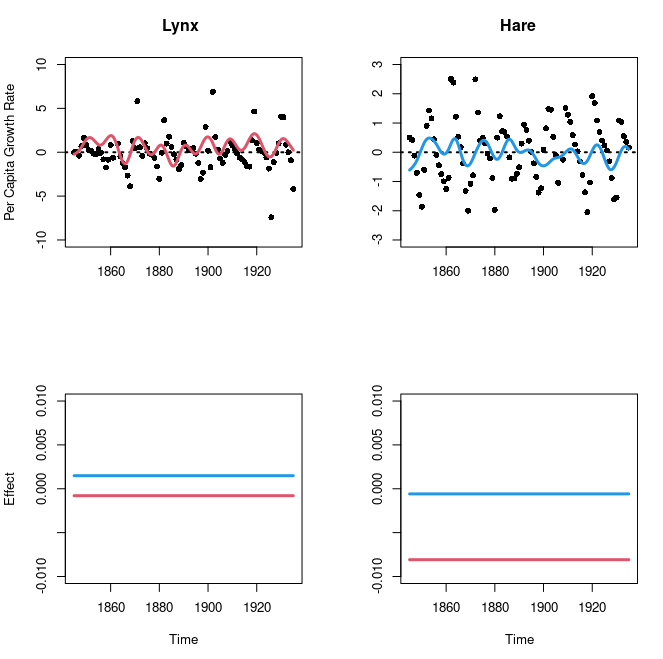
\includegraphics[width=\columnwidth]{lynxhareplot}}
\caption{
NODE results for the Lynx-Hare system and subsequent effects. The bottom plots represent the effects that the lynx (red) and hare (blue) have on a given population. Effect is measured as the partial derivative of the growth rate with respects to a given population
}
\end{center}
\end{figure}

\subsection{Laboratory Microcosm System}
Here we examine a three-species lab microcosm consisting of an algae \textit{Chlorella autrophica}, a flagellate \textit{Oxirrhis marina}, and a rotifer \textit{Brachionus plicatilis} \cite{tritropicpaper}. The flagellate eats the algae, and the rotifer eats both other microbes, though primarily the flagellate. Data points are measured daily. The system behaves ordinarily for a three species predator-prey system, with oscillations roughly every 3 weeks. Once again, we can look at the NODE plots in figure 2 (above). There is less noise in this system, which means the NODEs do a much better job fitting the data. We once again see that species generally don't affect their own growth rate. We can also see the standard predator-prey effects. Predators are affect positively by their prey and prey are affected very negatively by their predators. This would be a much more complicated system to fit by hand, but the NODE fitting has generated a simple system of differential equations that accounts for most of the growth rate.
\begin{figure}
\begin{center}
\centerline{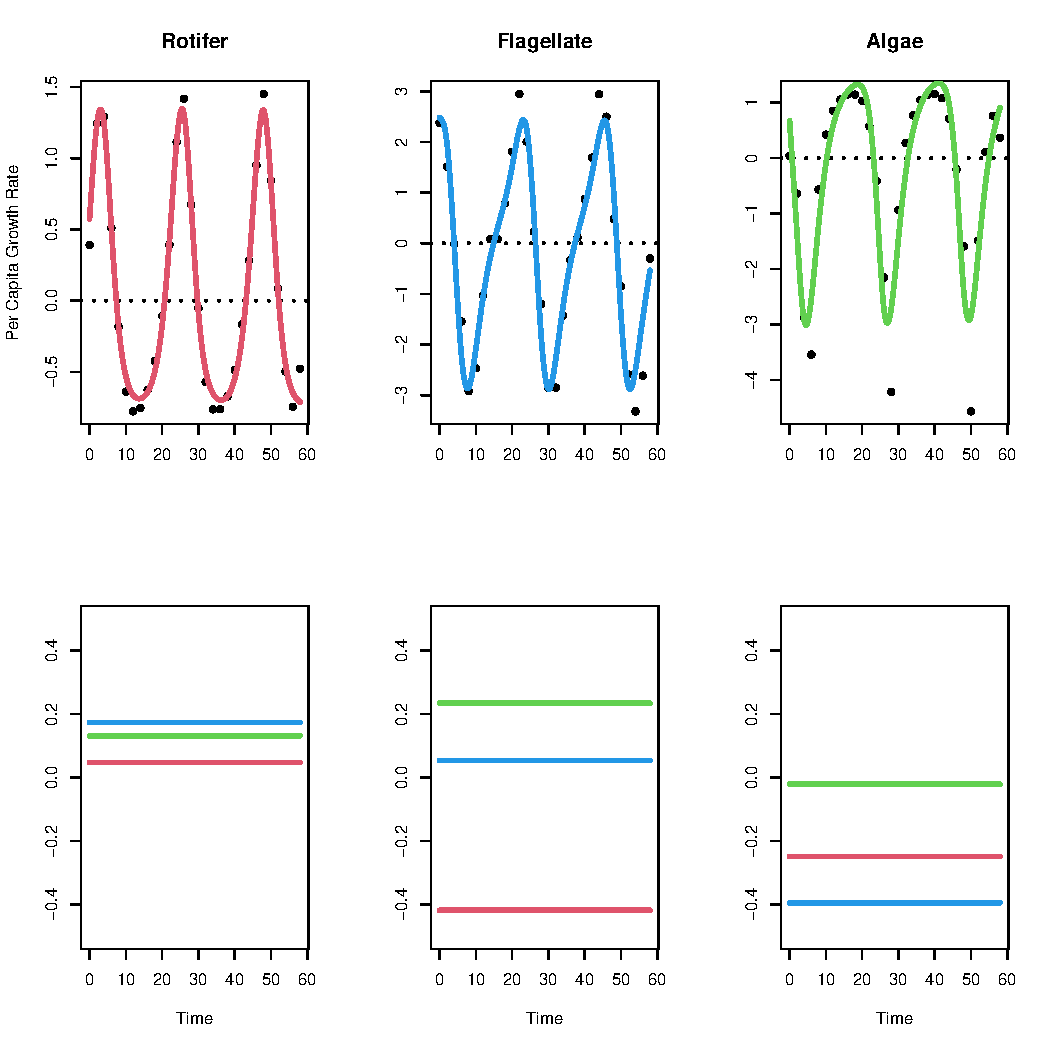
\includegraphics[width=\columnwidth]{tritropicplot}}
\caption{
NODE results for the microcosm and subsequent effects. The effects are plotted similarly to Figure 1
}
\end{center}
\end{figure}

\section{Discussion}
It can be really difficult and inefficient to find ecological relationships by testing parametric models against time series. NODEs provide an automated alternative that once implemented can be much faster. 

One exciting application of NODEs is on population dynamics over both time and space \cite{earlierpaper}. Since ANNs can be very flexible with their inputs and outputs, it would be feasible to extend the model to partial derivatives so that we can model dynamics in more than one dimension. The primary obsticle to this is the lack of good, precise data in time and space dimensions. As we saw in the lynx-hare system, small ANNs are very sensitive to noise in their data. 

This is one of the primary drawbacks to this method. This could potentially be dampened by adjusting the activation function. My primary goal for an activation function was simplicity, which is why I chose $f_\sigma(x)=x$. A different activation could be chosen to dampen the effects of noise in the data.

Another big drawback to this method is computational costs. This paper dealt with relatively small data sets with incredibly small ANNs. More data sets would provide more training, which could reveal more complex relationships, and large ANNs would be required to pick up on those relationships. There has been significant thrusts in optimizing this process, notably the BNGM process \cite{primarypaper}, which was brought up in the paper that inpired this one.

In conclusion, NODEs are a powerful new tool in the world of ecological modeling and have a lot of potential applications as they continue improving.

\bibliographystyle{sdss2020}
\bibliography{references}

\end{document}